\documentclass[tikz,border=2mm]{standalone}
\definecolor{structure}{HTML}{1A535C}
\definecolor{main}{HTML}{C6892A}
\definecolor{third}{HTML}{8B2635}

\begin{document}

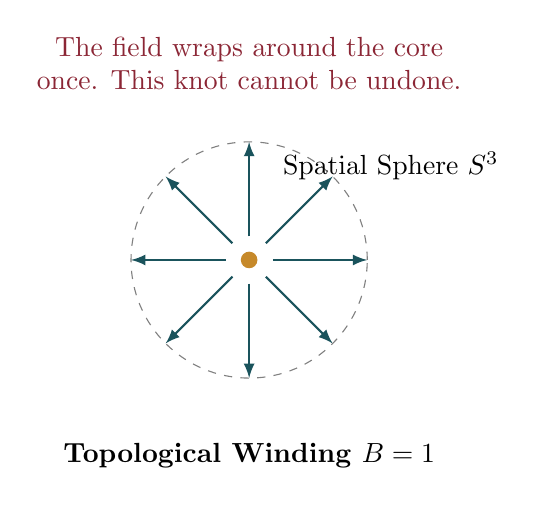
\begin{tikzpicture}[scale=1]

% Core
\fill[main] (0,0) circle (3pt);
\node[below=2mm] at (0,-2) {\textbf{Topological Winding $B=1$}};

% Hedgehog configuration — arrows radiating outward from centre
\foreach \angle in {0, 45, ..., 315} {
    \draw[->, thick, structure, >=latex] (\angle:0.3) -- (\angle:1.5);
}

% Dashed circle indicating the spatial S³ map
\draw[dashed, gray] (0,0) circle (1.5);
\node at (1.8, 1.2) {Spatial Sphere $S^3$};

% Annotation
\node[align=center, color=third] at (0, 2.5)
    {The field wraps around the core \\ once. This knot cannot be undone.};

\end{tikzpicture}

\end{document}
